\begin{figure}[h]
\centering
\begin{center}
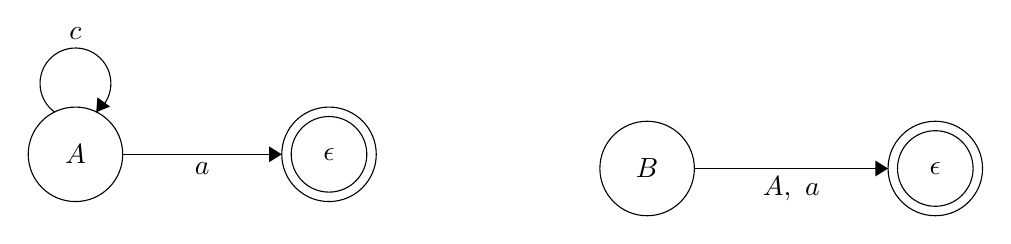
\begin{tikzpicture}[scale=0.2]
\tikzstyle{every node}+=[inner sep=0pt]
\draw [black] (11.2,-14.4) circle (3);
\draw (11.2,-14.4) node {$A$};
\draw [black] (47.5,-15.3) circle (3);
\draw (47.5,-15.3) node {$B$};
\draw [black] (65.8,-15.3) circle (3);
\draw (65.8,-15.3) node {$\epsilon$};
\draw [black] (65.8,-15.3) circle (2.4);
\draw [black] (27.3,-14.4) circle (3);
\draw (27.3,-14.4) node {$\epsilon$};
\draw [black] (27.3,-14.4) circle (2.4);
\draw [black] (9.877,-11.72) arc (234:-54:2.25);
\draw (11.2,-7.15) node [above] {$c$};
\fill [black] (12.52,-11.72) -- (13.4,-11.37) -- (12.59,-10.78);
\draw [black] (14.2,-14.4) -- (24.3,-14.4);
\fill [black] (24.3,-14.4) -- (23.5,-13.9) -- (23.5,-14.9);
\draw (19.25,-14.9) node [below] {$a$};
\draw [black] (50.5,-15.3) -- (62.8,-15.3);
\fill [black] (62.8,-15.3) -- (62,-14.8) -- (62,-15.8);
\draw (56.65,-15.8) node [below] {$A,\mbox{ }a$};
\end{tikzpicture}
\end{center}		
\decoRule
\caption[Conflicts in a graph]{Machine B has a conflict on encountering a terminal 'a'}
\label{fig:ConflictExample}
\end{figure}
